\documentclass[10pt,letterpaper]{article}
\usepackage[T1]{fontenc}
\usepackage{amssymb}
\usepackage{amsmath}
\usepackage{enumerate}
\usepackage[margin=0.5in]{geometry}
\usepackage{graphicx}
\usepackage{listings}
\usepackage{xcolor}

\definecolor{TangGreen}{HTML}{377459}

\lstset{
	basicstyle=\footnotesize\ttfamily,
	columns=flexible,
	breaklines=true,
	commentstyle=\color{TangGreen},
	keywordstyle=\color{black}\bfseries,
	keepspaces=true
}

\title{Numerical Computing Problem Set 2}
\author{Jeremy Chen}
\date{September 15, 2026}
\begin{document}
	\maketitle

\noindent \textbf{1. } (10 pts) The function $f(x) = \cos(3x) - \tanh(x)$ has two real roots in the interval $[-1, 1]$. 

\begin{enumerate}[\textbf{(\alph{enumi})}]

\item Graph the function using Matlab and include a graph with your solution. By evaluating the function $f(x) =$ at different values of $x$ (using Matlab or a calculator) find intervals [a, b] of (exactly) length 1/2 that bracket each root.

\begin{figure}[h!]
\centering
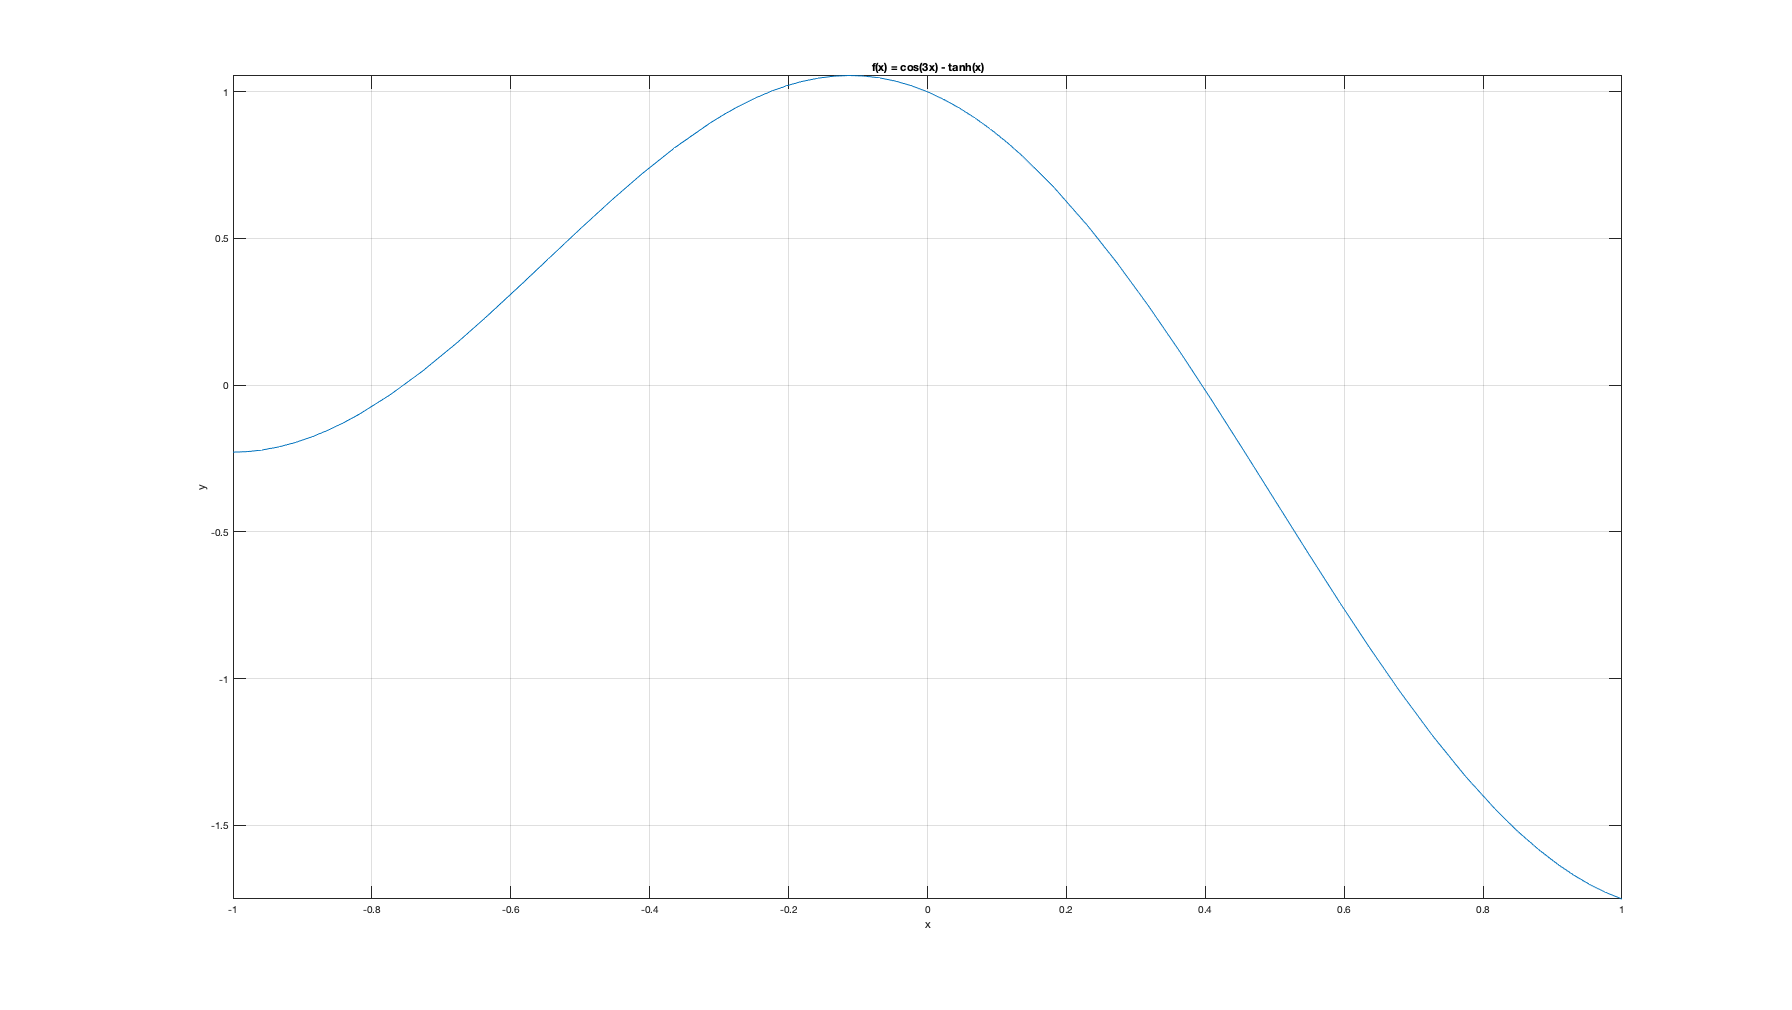
\includegraphics[width=0.7\linewidth]{Question 1 Plot.png}
\end{figure}

\color{TangGreen}
The intervals that bracket the roots are $[-1, -0.5]$ and $[0, 0.5]$. 
\color{black}

\item Estimate how many iterations the bisection method will need to find each root correct to 10 decimal places.

\color{TangGreen}
Using the solution error inequality (1.1), the following could be constructed
$$\frac{1}{2^{n + 1}} < 0.5 * 10^{-10}$$
Reformulating this would result in the following
$$n > \frac{10}{\log_{10}2} \approx 33.2$$
meaning that there would need to be at least 34 iterations. 
\color{black}

\end{enumerate}

\noindent \textbf{2. } (20 pts) Implement the bisection method in a Matlab function:

\noindent{\tt \% bisect: find an approximate solution to f(x)=0 using bisection\\
\%\\
\% f(input) : function f(x)\\
\% a,b (input) : interval to search that brackets the root, a<b and f(a)*f(b) <= 0\\
\% tol (input) : tolerance\\
\% maxIterations (input) : maximum number of iterations allowed\\
\% xc (output) : approximate solution\\
function xc = bisect( f, a, b, tol, maxIterations)}

\noindent(e.g. you could base your code on Program 1.1, {\tt bisect}, from the text, but some changes are needed as noted next). 

\begin{itemize}

\item Iterate until $|(b - a) / 2| <$ {\tt tol}

\item Keep track of the iteration number, $k$, and take at most {\tt maxIterations} iterations. Print an error message if the maximum number of iterations is exceeded. 

\item Add a statement to the code that outputs the current values for $a_{k}, f(a_{k}), b_{k}, f(b_{k})$ and $c_{k}$ at iteration $k = 1, 2, \dots$. You could use the following statements:

{\tt fprintf('bisect: k=\%2d, a=\%11.4e f(a)=\%8.2e b=\%11.4e f(b)=\%8.2e c=\%14.7e\textbackslash n’,k,a,fa,b,fb,c);}

\end{itemize}

\noindent Use your {\tt bisect} function to find three real roots of the following equation on the interval [-1, 1.5],
$$f(x) = \cos(3x) + 0.5x^{3}$$
Plot the function in Matlab and determine starting intervals $[a, b]$ of length 1 hat bracket each root (provide the plot with your answer). Use the bisection function to determine each root using {\tt tol}$= 10^{-6}$ and {\tt maxIterations}$= 100$. Include the output from the {\tt bisect} routine.

\color{TangGreen}
The following is the code for the modified bisect function.

\lstinputlisting[language=Matlab, numbers=left, stepnumber=1, firstline=1,caption={bisect2.m, Modified bisection function},label=code:bisection modified,frame=single]{bisect2.m}

The three intervals that bracket the roots are $[-1, 0]$, $[0, 1]$, and $[0.6, 1.6]$. The following are the outputs for the bisection 

\begin{lstlisting}[frame=single,caption={The first root},label=root1]
>> root1 = bisect2(f, a, b, tol, 100)
bisect: k=19, a=-5.0245e-01 f(a)=-3.37e-06 b=-5.0244e-01 f(b)=3.06e-06 c=-5.0244331e-01

root1 =

   -0.5024
\end{lstlisting}
\begin{lstlisting}[frame=single,caption={The second root},label=root2]
>> root2 = bisect2(f, a, b, tol, 100)
bisect: k=19, a= 5.5160e-01 f(a)=2.30e-06 b= 5.5161e-01 f(b)=-2.53e-06 c= 5.5160332e-01

root2 =

   0.5516
\end{lstlisting}
\begin{lstlisting}[frame=single,caption={The third root},label=root3]
>> root3 = bisect2(f, a, b, tol, 100)
bisect: k=19, a= 1.2092e+00 f(a)=-3.57e-06 b= 1.2093e+00 f(b)=3.29e-06 c= 1.2092510e+00

root3 =

   1.2093
\end{lstlisting}

And the following is the plot produced by Matlab for the given $f(x)$. 
\begin{figure}[h!]
	\centering
	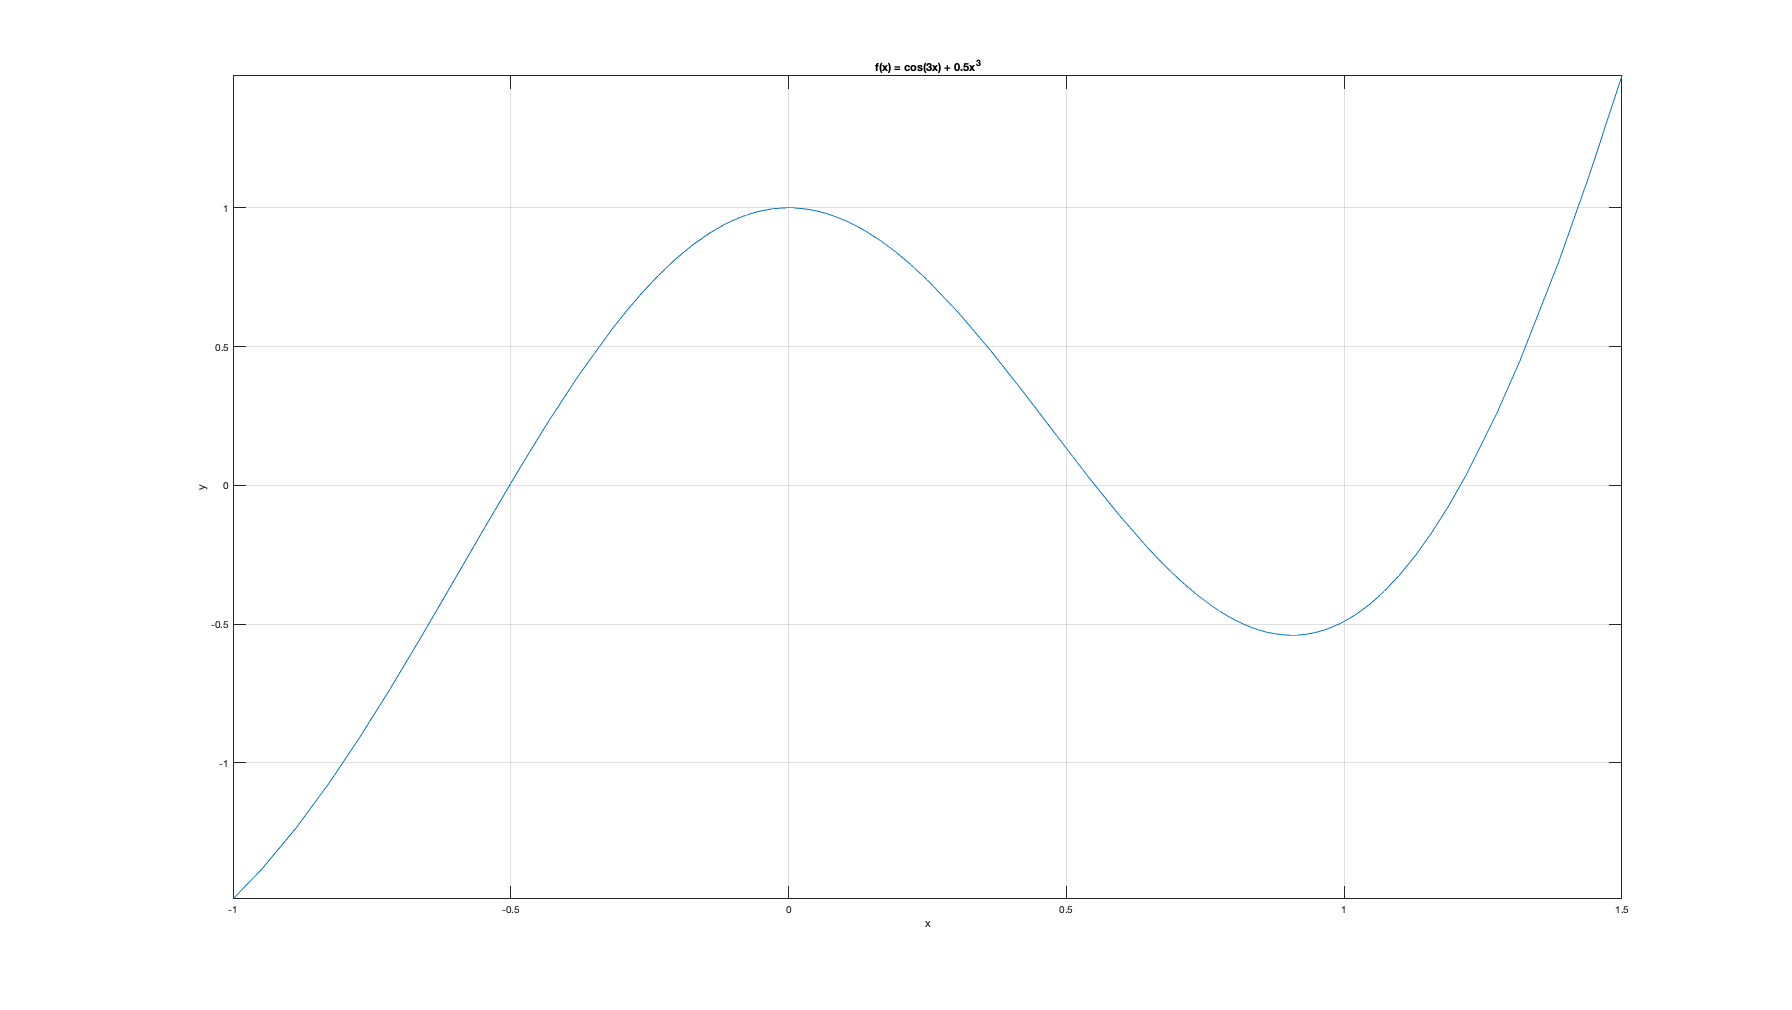
\includegraphics[width=0.7\linewidth]{Question 2 Plot.png}
\end{figure}
\color{black}

\noindent \textbf{3.} (10 pts) Consider solving the equation $f(x) = 0$ using a fixed-point iteration $x_{k + 1} = g(x_{k})$ to solve $x = g(x)$ for a root $x = r$. 

For each of the following, find the fixed points analytically and use the convergence analysis for fixed point iterations to determine whether the fixed point iteration will converge (given a good enough initial guess). For the cases that converge, what is the asymptotic convergence rate?

\begin{enumerate}[\textbf{(\alph{enumi})}]

\item $g(x) = x^{2} + \frac{1}{6}x + \frac{1}{6}$

\color{TangGreen}
$g(x)$ could be reformulated as the following
$$x^{2} + \frac{1}{6}x + \frac{1}{6} = 0 \rightarrow x^{2} = -\frac{1}{6} - \frac{1}{6}x \rightarrow x = \sqrt{-\frac{1}{6} - \frac{1}{6}x}$$
$g(x)$ does not converge. 
\color{black}

\item $g(x) = \frac{1}{2}x^{2} - \frac{1}{2}x + 1$

\color{TangGreen}
$g(x)$ here could be reformulated as
$$\frac{1}{2}x^{2} - \frac{1}{2}x + 1 = 0 \rightarrow \frac{1}{2}x^{2} = \frac{1}{2}x - 1 \rightarrow x^{2} = x - 2 \rightarrow x = \sqrt{x - 2}$$
Here, $g(x)$ converges at -2. Given definition (1.11), the asymptotic convergence rate is
$$|g'(r)| \rightarrow S = \left| \frac{1}{2 \sqrt{-2 - 2}} \right| = \frac{i}{4}$$
\color{black}

\end{enumerate}

\noindent \textbf{4.} (20 pts) Implement the fixed point iteration in a Matlab function {\tt fixedPoint}:

{\tt \% Compute a fixed point g(x) = x\\
\indent \% \ \ g \ (input) : function to use\\
\indent \% \ \ x0 (input) : initial guess\\
\indent \% \ \ tol (input) : convergence tolerance\\
\indent \% \ \ maxIterations (input) : maximum number of iterations\\
\indent \% \ \ xc (output) : approximation to the fixed point\\
\indent function xc = fixedPoint( g, x0, tol, maxIterations )}
\begin{itemize}

\item Include a statement in the function to print the iteration number k, the current approximation, $x_{k + 1}$, and $|x_{k + 1} - x_{k}|$. For example:

{\tt fprintf(’fixedPoint: k=\%2d xc=\%18.12e |xc-xOld|=\%8.2e\textbackslash n’,k,xc,abs(xc-xOld))}

\item Iterate until $|x_{k + 1} - x_{k}| <$ {\tt tol} or the number of iterations has exceed {\tt maxIterations}.

\item Print an error message if the iteration did not converge after {\tt maxIterations}. 

\end{itemize}
Use your {\tt fixedPoint} function to find an approximation to the real root of the function
$$f(x) = 3x^{3} + x + 1$$
using the following fixed point iterations,

\begin{enumerate}[(a)]

\item $g(x) = \left( (1 - x)/3 \right)^{1/3}$

\item $g(x) = 1 - 3x^{3}$

\item $g(x) = (1 + 6x^{3}) / (1 + 9x^{2})$

\end{enumerate}
In each case, use a starting guess of $x_{0} = 0.6$. Compute the solution using {\tt tol}$= 10^{-5}$ and {\tt maxIterations}=20. Explain why the iteration converged or did not converge, based on the convergence theory. 

\color{TangGreen}
The modified FPI code is the following
\lstinputlisting[language=Matlab, numbers=left, stepnumber=1, firstline=1,caption={fpi2.m, Modified FPI function},label=code:FPI modified,frame=single]{fpi2.m}
The following are the code executions for the three forms of $g(x)$
\begin{lstlisting}[frame=single,caption={$g(x) = ((1 - x)  3)^{1/3}$},label=FPI1]
>> xc = fpi2(g, x0, tol, maxIterations)

xc =

   0.5366
\end{lstlisting}
\begin{lstlisting}[frame=single,caption={$g(x) = 1 - 3x^{3}$},label=FPI2]
>> xc = fpi2(g, x0, tol, maxIterations)
Error using fpi2
Exceeded max iterations
\end{lstlisting}
\begin{lstlisting}[frame=single,caption={$g(x) = (1 + 6x^{3}) / (1 + 9x^{2})$},label=FPI3]
>> xc = fpi2(g, x0, tol, maxIterations)

xc =

   0.5366
\end{lstlisting}
The reason that the second $g(x)$ didn't converge is because $|g'(r)|$ is equal to -2.59, which has an absolute value greater than 1. The first $g(x)$ has convergence rate 0.385 and the third $g(x)$ has convergence rate of 0.0000937. 
\color{black}

\end{document}